\chapter{Results}\label{chap:results}

In the scope of this thesis, the main focus was on binary classification models. While we did explore regression models, the primary findings are derived from evaluation of the classification models and thus omitted the regression results.

\section{Binary Classification}
In the context of prioritizing compounds based on hazard assessment, the objective is to maximize the probability of detecting toxic compounds while minimizing the the number of false alarms, which represent non-hazardous compounds misclassified as toxic. Initially, we introduce the performance metrics used for model evaluation.

\subsection{Evaluation Metrics}
When assessing the performance of a binary prediction model with a validation dataset containing known target values, four key quantities come into play (and presented as Confusion Matrix in Table~\ref{tab:confusion_matrix}):

\begin{table}[h]
  \centering
  \small
  \caption{Confusion Matrix}
  \label{tab:confusion_matrix}
  \setlength{\tabcolsep}{10pt} % Adjust cell padding
  \renewcommand{\arraystretch}{1.5} % Adjust cell height
  \begin{tabular}{|c|c|c|}
  \cline{2-3}
  \multicolumn{1}{c|}{} & Actual Negative & Actual Positive \\
  \hline
  Predicted Negative & TN & FN \\
  \hline
  Predicted Positive & FP & TP \\
  \hline
  \end{tabular}
\end{table}

\begin{itemize}
  \item True Positives (TP): The number of correctly predicted active cases.
  \item True Negatives (TN): The number of correctly predicted inactive cases.
  \item False Positives (FP): The number of incorrectly predicted active cases.
  \item False Negatives (FN): The number of incorrectly predicted inactive cases.
\end{itemize}

The classification threshold is a crucial parameter dictating how the model assigns data points to one of two classes based on predicted class probabilities. This threshold significantly influences the model's metrics, as illustrated in Figure~\ref{fig:classification_threshold} and showcased in Figure~\ref{fig:roc1120} and Figure~\ref{fig:cm1120}.
\begin{figure}[h]
  \centering
  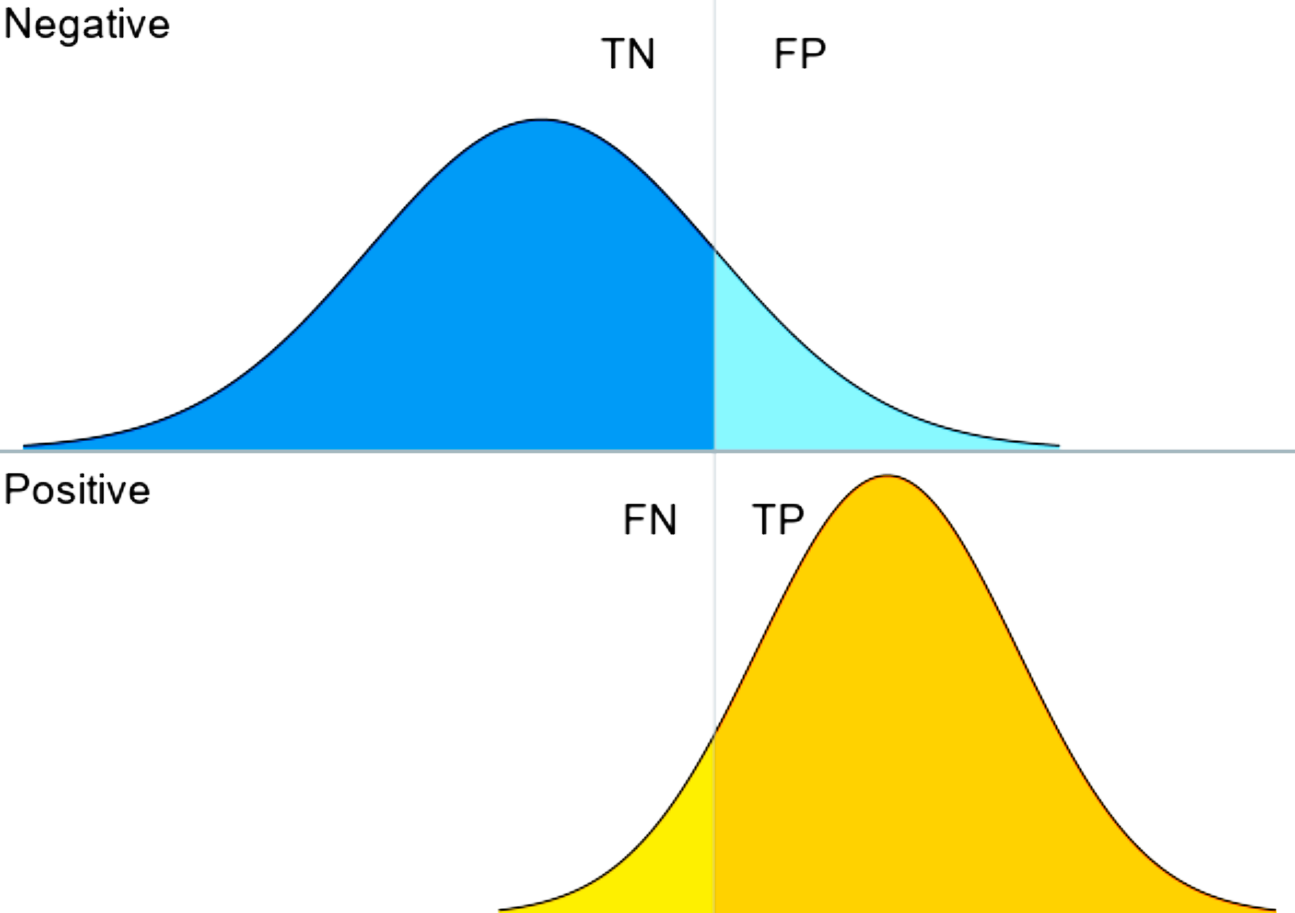
\includegraphics[width=0.5\textwidth]{figures/classification_threshold.png}
  \caption{Relationship between threshold and classification. Figure obtained from~\cite{wicklin2020}}
~\label{fig:classification_threshold}
\end{figure}

Various metrics assess predictive model performance, such as:

\begin{itemize}
  \item \textbf{Accuracy} is the ratio of correctly classified instances (TP) and (TN) to the total number of instances. It provides a general measure of the model's correctness.
  \[ \text{Accuracy}  A = \frac{TP + TN}{TP + TN + FP + FN} \]

  \item \textbf{Precision (P)} is the proportion of correctly predicted active cases (TP) to all instances predicted as active (TP + FP). 
  \[ \text{Precision } P = \frac{TP}{TP + FP} \]

  \item \textbf{Recall (R) or Sensitivity or True Positive Rate (TPR)} is the proportion of correctly predicted active cases (TP) to all actual active cases (TP + FN).
  \[ \text{Recall } R = \frac{TP}{TP + FN} \]

  \item \textbf{F1 Score} is the harmonic mean of precision and recall, which balances the trade-off between false positives and false negatives.
  \[ F1 = \frac{2 \cdot P \cdot R}{P + R} \]

  \item \textbf{True Negative Rate (TNR) or Specificity} is the proportion of correctly predicted inactive cases (TN) to all actual inactive cases (TN + FP).
  \[ TNR = \frac{TN}{TN + FP} \]

  \item \textbf{Receiver Operating Characteristic (ROC) Curve} is a graphical representation of the model's performance across different classification thresholds and plots the true positive rate (TNR) against the false positive rate (FPR), as exemplified for assay endpoint with $aeid=1120$ in Figure~\ref{fig:roc1120}. The Area Under the ROC Curve (AUC) is an indicator of the model's performance taking into acount all possible classification thresholds, where a score of 1 represents a perfect model and 0.5 signifies a random no-skill model. 


\end{itemize}

\begin{figure}[h]
  \centering
  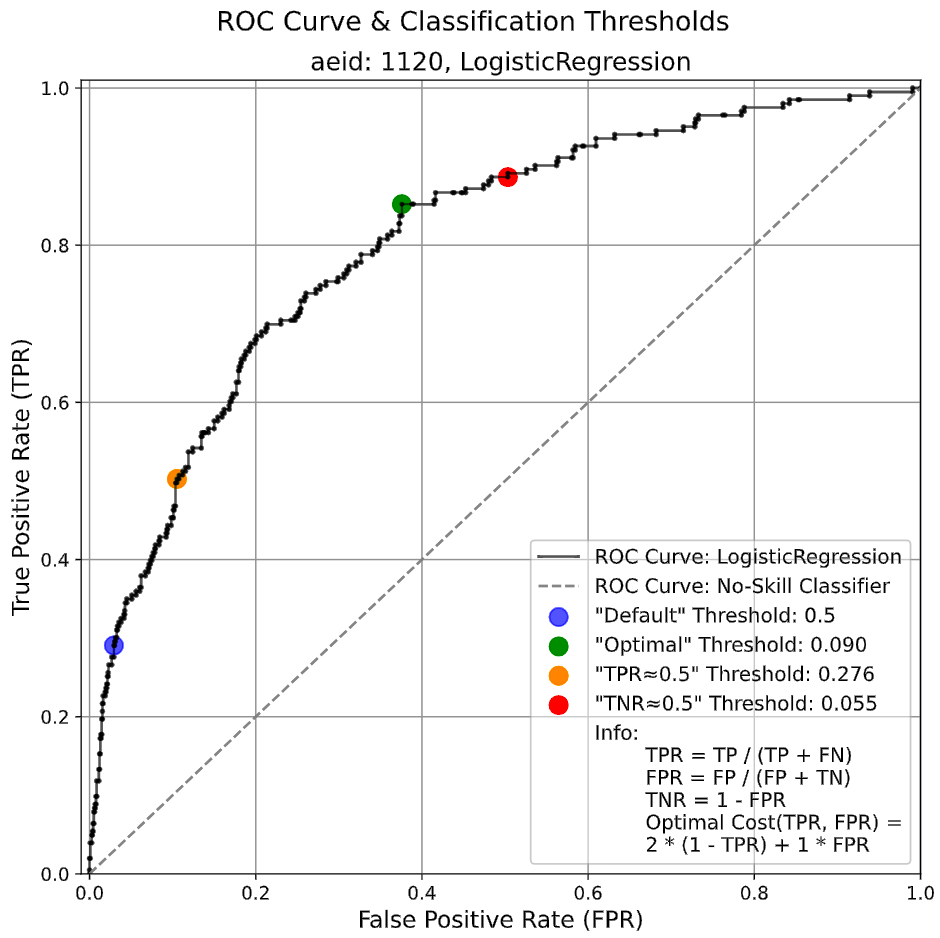
\includegraphics[width=0.6\textwidth]{figures/roc1120.png}
  \caption{The Receiver Operating Characteristic (ROC) curve is presented for the LogisticRegression classifier in the case of assay endpoint with aeid: 1120. We make predictions for each model combination using four distinct classification thresholds, specifically: the default threshold of 0.5, the optimal threshold determined by the cost function weighting TPR twice as FPR (to value recall), TPR approximately equal to 0.5, and TNR approximately equal to 0.5. Figure~\ref{fig:cm1120} shows the confusion matrices for the four thresholds.}
~\label{fig:roc1120}
\end{figure}

\begin{figure}[h]
  \centering
  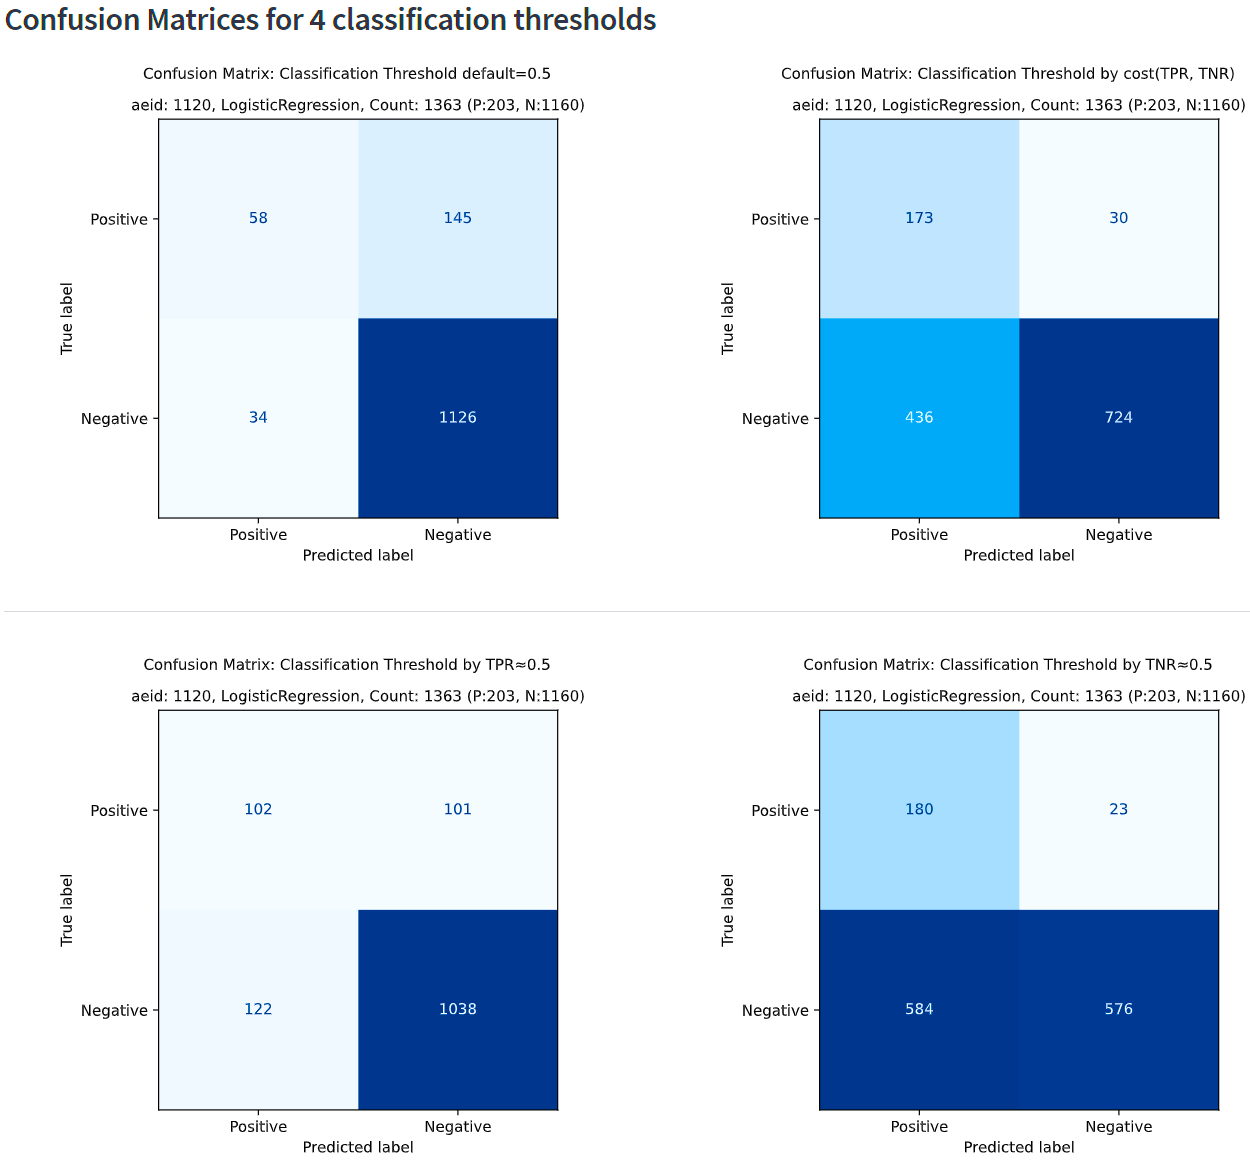
\includegraphics[width=1.0\textwidth]{figures/cm1120.png}
  \caption{For assay endpoint with aeid: 1120, confusion matrices are shown for four different classification thresholds.}
~\label{fig:cm1120}
\end{figure}

\subsubsection{Imbalanced Data}
A substantial proportion of the studied assay endpoints have an unequal distribution of active (positive) and inactive (negative) compounds. Typically, the negative class significantly outweights the positive class, as depicted by an example in Figure~\ref{fig:cm1120}. Such imbalanced datasets can result in skewed performance metrics, where the model may exhibit strong performance on the majority class while performing poorly on the minority class. To address imbalanced datasets, additional metrics such as macro averaged and weighted averaged metrics can be taken into account.
In macro-averaging, individual class metrics are calculated and then equally weighted to compute an overall metric, disregarding class distribution. For instance, macro recall is the average of individual class recalls:
\[
\text{Macro Recall } = \frac{R_{positive} + R_{neagtive}}{2}
\]
In weighted averaging, individual class metrics are calculated and then weighted by the number of true instances in each class. For instance, weighted recall is the average of individual class recalls weighted by the number of true instances in each class. Similarly macro-averaged and weighted-averaged precision and F1 score can be calculated. The following two metric scores are not directly dependent on the threshold, and thus are well-suited for comparing models with imbalanced datasets:

\begin{itemize}
  \item \textbf{Balanced Accuracy (BAC)} accounts for class imbalance by averaging the true positive rate (sensitivity) and true negative rate (specificity).
  \[ \text{Balanced Accuracy (BAC)} = \frac{1}{2} \left(\frac{TP}{TP + FN} + \frac{TN}{TN + FP}\right) \]

  \item \textbf{PR-AUC (Precision-Recall Area Under the Curve)} quantifies the performance of the positive class by assessing the area under the precision-recall curve.
  
\end{itemize}



\subsection{Performance}\label{sec:performance}

Performance results were generated for every combination of:

\begin{itemize}
  \item Target variables (y):
  \begin{enumerate}
    \item hitcall without cytotoxicity correction
    \item hitcall with cytotoxicity correction
  \end{enumerate}
  \item 345 Assay endpoints:
  \item Feature selection (FS) models:
    \begin{enumerate}
      \item XGBoost
      \item RandomForest
    \end{enumerate}
    \item Estimator models:
    \begin{enumerate}
      \item LogisticRegression
      \item MLPClassifier
      \item RandomForestClassifier
      \item SVM (Support Vector Machine)
      \item XGBoostClassifier
    \end{enumerate}
  \item Validation sets:
    \begin{enumerate}
      \item the internal validation dataset 
      \item MassBank validation set with fingerprints from chemical structure
      \item MassBank validation set with SIRIUS-predicted fingerprints
    \end{enumerate}
  \item Classification thresholds:
    \begin{enumerate}
      \item $default$: classification threshold of 0.5
      \item $TPR \simeq 0.5$: TPR approximately equal to 0.5. In other words, the threshold is chosen such that the models detect approximately $50\%$ of the toxic compounds. This choice provides an estimate on the price to pay in terms of false positives, facilitating performance comparisons with other models.
      \item $TNR \simeq 0.5$: TNR approximately equal to 0.5.
      \item $\text{cost}(TPR, TNR)$: cost function weighting TPR twice as FPR: the threshold is chosen such that $\text{cost}(TPR, TNR) = 2 * (1 - TPR) + FPR$ is minimized, valueing recall twice as precision.
    \end{enumerate}
  \item Metrics on: 1. macro average, 2. weighted average, 3. positive and 4. negative class
\end{itemize}

Below, we present a selection of these outcomes in the form of figures and summary tables, showcasing the performance of binary classification models with the following fixed configurations:
\begin{itemize}
  \item binarized hitcall without cytotoxicity correction as the target variable
  \item XGBoost as the feature selection model
  \item macro averaged metrics
\end{itemize}

With these settings, we evaluated the performance across all assay endpoints and estimators on the internal validation set the dual MassBank validation set. Note that reproted balanced accuracy, the ROC-AUC and PR-AUC metric scores remain consistent across subsequent summaries, unaffected by the choice of classification threshold. The figures are presented in the following order:

\begin{table}[h]
  \centering
  \caption{Figure References and Descriptions}
  \small
  \begin{tabular}{lll}
    \toprule
    \textbf{Validation set} & \textbf{Classification Threshold} & \textbf{Figure} \\
    \midrule
    \small Internal & \small $default = 0.5$ & \small Figure~\ref{fig:hitcall_classification_Feature_Selection_XGBClassifier_val_default_macro_avg} \\
    \small Internal & \small $\text{cost}(TPR, TNR) = 2 \cdot (1 - TPR) + FPR$ & \small Figure~\ref{fig:hitcall_classification_Feature_Selection_XGBClassifier_val_optimal_macro_avg} \\
    \small Internal & \small $TPR \simeq 0.5$ & \small Figure~\ref{fig:hitcall_classification_Feature_Selection_XGBClassifier_val_tpr_macro_avg} \\
    \small Internal & \small $TNR \simeq 0.5$ & \small Figure~\ref{fig:hitcall_classification_Feature_Selection_XGBClassifier_val_tnr_macro_avg} \\
    \midrule
    \small MassBank from structure & \small $default = 0.5$ & \small Figure~\ref{fig:hitcall_classification_Feature_Selection_XGBClassifier_mb_val_structure_default_macro_avg} \\
    \small MassBank SIRIUS-predicted & \small $default = 0.5$ & \small Figure~\ref{fig:hitcall_classification_Feature_Selection_XGBClassifier_mb_val_sirius_default_macro_avg} \\
    \small MassBank from structure & \small $\text{cost}(TPR, TNR) = 2 \cdot (1 - TPR) + FPR$ & \small Figure~\ref{fig:hitcall_classification_Feature_Selection_XGBClassifier_mb_val_structure_optimal_macro_avg} \\
    \small MassBank SIRIUS-predicted & \small $\text{cost}(TPR, TNR) = 2 \cdot (1 - TPR) + FPR$ & \small Figure~\ref{fig:hitcall_classification_Feature_Selection_XGBClassifier_mb_val_sirius_optimal_macro_avg} \\
    \small MassBank from structure & \small $TPR \simeq 0.5$ & \small Figure~\ref{fig:hitcall_classification_Feature_Selection_XGBClassifier_mb_val_structure_tpr_macro_avg} \\
    \small MassBank SIRIUS-predicted & \small $TPR \simeq 0.5$ & \small Figure~\ref{fig:hitcall_classification_Feature_Selection_XGBClassifier_mb_val_sirius_tpr_macro_avg} \\
    \small MassBank from structure & \small $TNR \simeq 0.5$ & \small Figure~\ref{fig:hitcall_classification_Feature_Selection_XGBClassifier_mb_val_structure_tnr_macro_avg} \\
    \small MassBank SIRIUS-predicted & \small $TNR \simeq 0.5$ & \small Figure~\ref{fig:hitcall_classification_Feature_Selection_XGBClassifier_mb_val_sirius_tnr_macro_avg} \\
    \bottomrule
  \end{tabular}
\end{table}

\newpage


\subsubsection{Internal Validation Set}\label{sec:internal_validation_set}

\begin{figure}[h]
  \centering
  \begin{subfigure}[b]{0.495\textwidth}
      \centering
      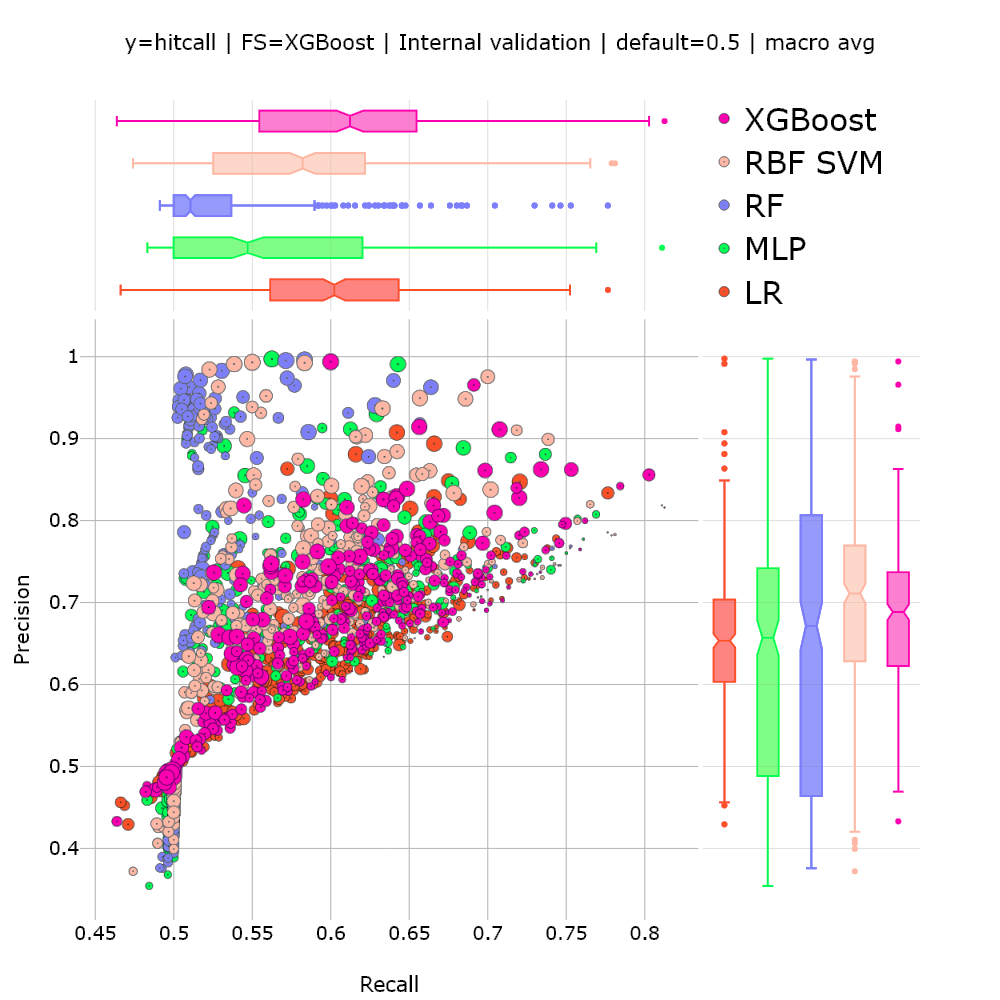
\includegraphics[width=\textwidth]{generated_results/hitcall_classification_Feature_Selection_XGBClassifier_val_default_macro_avg.png}
      \caption{}
  \label{fig:hitcall_classification_Feature_Selection_XGBClassifier_val_default_macro_avg}
  \end{subfigure}
  \hfill
  \begin{subfigure}[b]{0.495\textwidth}
      \centering
      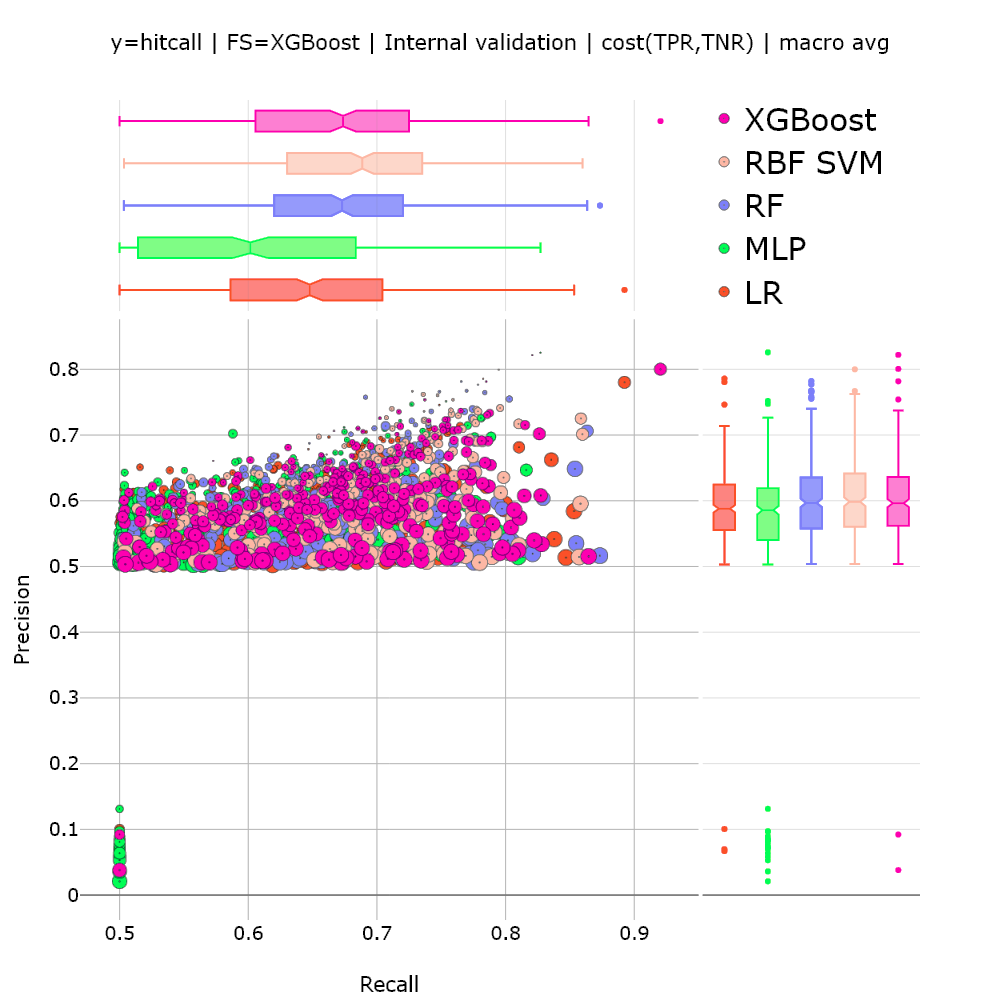
\includegraphics[width=\textwidth]{generated_results/hitcall_classification_Feature_Selection_XGBClassifier_val_optimal_macro_avg.png}
      \caption{}
      \label{fig:hitcall_classification_Feature_Selection_XGBClassifier_val_optimal_macro_avg}
  \end{subfigure}
  \caption{Comparison of precision and recall for five different estimators across a total of 345 evaluated assay endpoints for the \emph{internal validation set} (a)  $default = 0.5$  (b) $\text{cost}(TPR, TNR) = 2 * (1 - TPR) + FPR$ threshold. Larger marker size indicate a larger relative imbalance between the support for negative and positive compounds, normalized across all assay endpoints. The marginal boxplots illustrate the metric distribution across the target assay endpoint models (median, first quartile, third quartile, range-whiskers and outlieres). The tables below provide the median metrics for the estimators across all target assay endpoint models.}
  \label{fig:hitcall_classification_Feature_Selection_XGBClassifier_val_default_optimal_macro_avg}
\end{figure}


\begin{longtable}{llllllll}
\caption{Median Performance Metrics belonging to Figure~\ref{fig:hitcall_classification_Feature_Selection_XGBClassifier_val_default_macro_avg}.}\label{tab:table:hitcall_classification_feature_selection_xgbclassifier_val_default_macro_avg}\\
\toprule
\midrule
\small Estimator & \small Precision & \small Recall & \small F1 & \small Acc. & \small Bal. Acc. & \small ROC-AUC & \small PR-AUC\\
\hline
LR & 0.653 & 0.602 & 0.617 & 0.827 & 0.602 & 0.711 & 0.367\\
MLP & 0.657 & 0.547 & 0.547 & 0.844 & 0.547 & 0.678 & 0.339\\
RBF SVM & 0.711 & 0.582 & 0.592 & 0.845 & 0.582 & 0.754 & 0.421\\
RF & 0.671 & 0.511 & 0.491 & 0.846 & 0.511 & 0.744 & 0.392\\
XGBoost & 0.688 & 0.612 & 0.632 & 0.837 & 0.612 & 0.741 & 0.417\\
\bottomrule
\end{longtable}
\begin{longtable}{llllllll}
\caption{Median Performance Metrics belonging to~\ref{fig:hitcall_classification_Feature_Selection_XGBClassifier_val_optimal_macro_avg}.}\label{tab:table:hitcall_classification_feature_selection_xgbclassifier_val_optimal_macro_avg}\\
\toprule
\midrule
\small Estimator & \small Precision & \small Recall & \small F1 & \small Acc. & \small Bal. Acc. & \small ROC-AUC & \small PR-AUC\\
\hline
LR & 0.588 & 0.648 & 0.440 & 0.496 & 0.602 & 0.711 & 0.367\\
MLP & 0.586 & 0.602 & 0.385 & 0.398 & 0.547 & 0.678 & 0.339\\
RBF SVM & 0.598 & 0.689 & 0.510 & 0.559 & 0.582 & 0.754 & 0.421\\
RF & 0.597 & 0.673 & 0.469 & 0.528 & 0.511 & 0.744 & 0.392\\
XGBoost & 0.596 & 0.674 & 0.496 & 0.553 & 0.612 & 0.741 & 0.417\\
\bottomrule
\end{longtable}
\newpage

\begin{figure}
\centering
\begin{subfigure}[b]{0.495\textwidth}
  \centering
  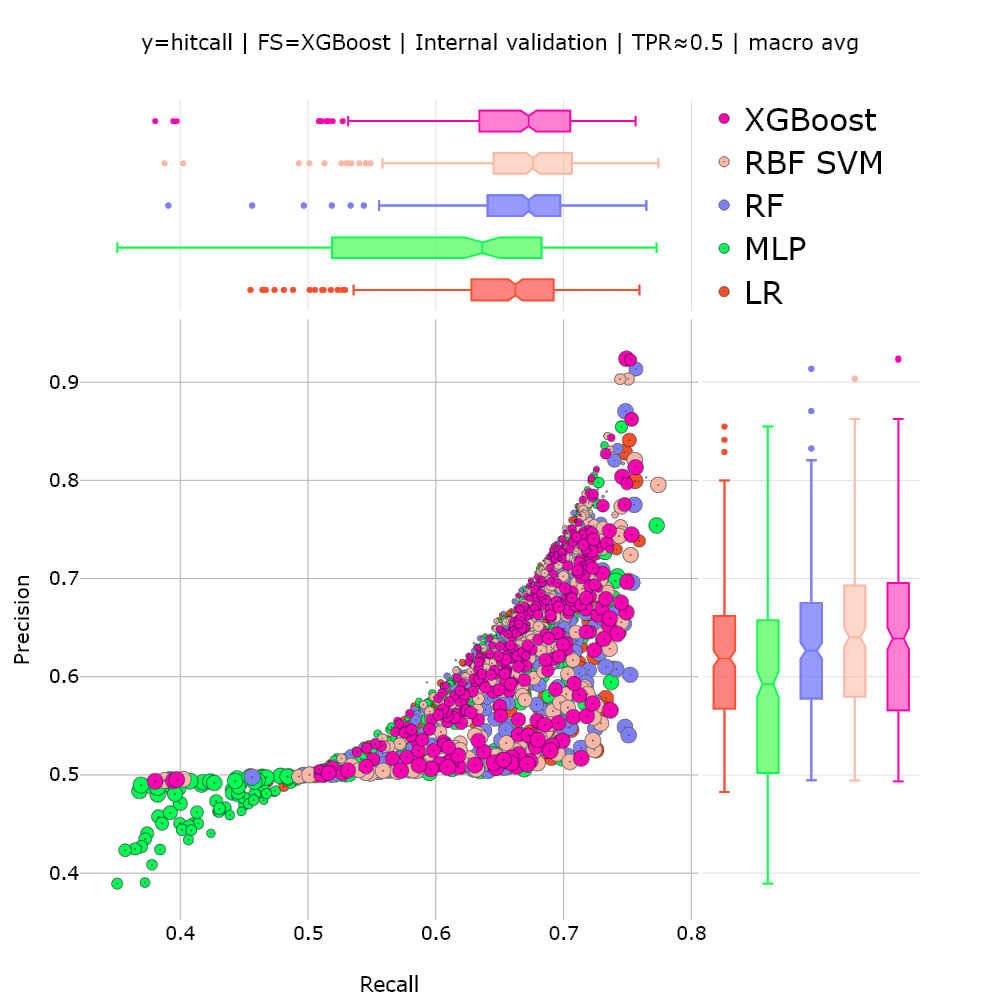
\includegraphics[width=\textwidth]{generated_results/hitcall_classification_Feature_Selection_XGBClassifier_val_tpr_macro_avg.png}
  \caption{}
\label{fig:hitcall_classification_Feature_Selection_XGBClassifier_val_tpr_macro_avg}
\end{subfigure}
\hfill
\begin{subfigure}[b]{0.495\textwidth}
  \centering
  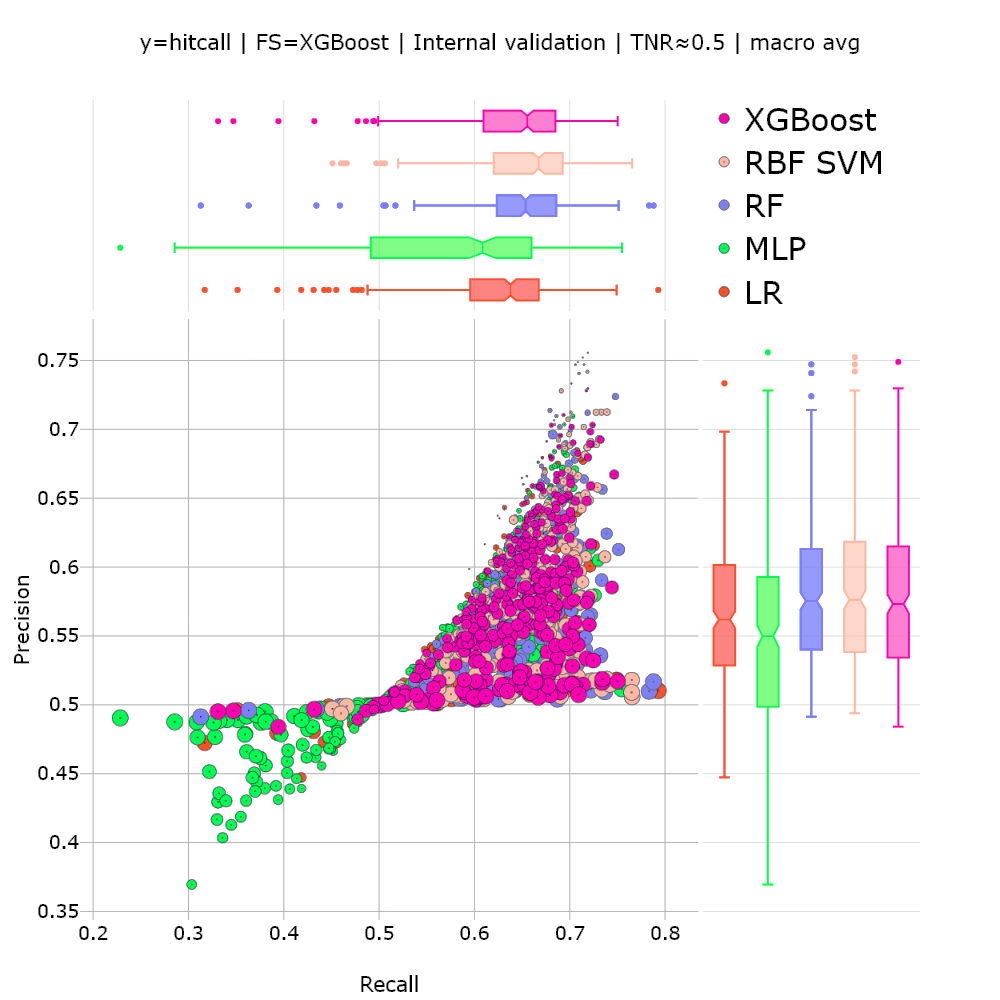
\includegraphics[width=\textwidth]{generated_results/hitcall_classification_Feature_Selection_XGBClassifier_val_tnr_macro_avg.png}
  \caption{}
  \label{fig:hitcall_classification_Feature_Selection_XGBClassifier_val_tnr_macro_avg}
\end{subfigure}
\caption{Comparison of precision and recall for five different estimators across a total of 345 evaluated assay endpoints for the \emph{internal validation set} (a) $TPR \simeq 0.5$ (b) $TNR \simeq 0.5$ classifiaction threshold. Larger marker size indicate a larger relative imbalance between the support for negative and positive compounds, normalized across all assay endpoints. The marginal boxplots illustrate the metric distribution across the target assay endpoint models (median, first quartile, third quartile, range-whiskers and outlieres). The tables below provide the median metrics for the estimators across all target assay endpoint models.}
\label{fig:hitcall_classification_Feature_Selection_XGBClassifier_val_default_optimal_macro_avg}
\end{figure}

\begin{longtable}{llllllll}
\caption{Median Performance Metrics belonging to Figure~\ref{fig:hitcall_classification_Feature_Selection_XGBClassifier_val_tpr_macro_avg}.}\label{tab:table:hitcall_classification_feature_selection_xgbclassifier_val_tpr_macro_avg}\\
\toprule
\midrule
\small Estimator & \small Precision & \small Recall & \small F1 & \small Acc. & \small Bal. Acc. & \small ROC-AUC & \small PR-AUC\\
\hline
LR & 0.619 & 0.662 & 0.632 & 0.746 & 0.602 & 0.711 & 0.367\\
MLP & 0.592 & 0.636 & 0.597 & 0.702 & 0.547 & 0.678 & 0.339\\
RBF SVM & 0.640 & 0.676 & 0.650 & 0.771 & 0.582 & 0.754 & 0.421\\
RF & 0.627 & 0.673 & 0.639 & 0.765 & 0.511 & 0.744 & 0.392\\
XGBoost & 0.639 & 0.673 & 0.649 & 0.763 & 0.612 & 0.741 & 0.417\\
\bottomrule
\end{longtable}
\begin{longtable}{llllllll}
\caption{Median Performance Metrics belonging to~\ref{fig:hitcall_classification_Feature_Selection_XGBClassifier_val_tnr_macro_avg}.}\label{tab:table:hitcall_classification_feature_selection_xgbclassifier_val_tnr_macro_avg}\\
\toprule
\midrule
\small Estimator & \small Precision & \small Recall & \small F1 & \small Acc. & \small Bal. Acc. & \small ROC-AUC & \small PR-AUC\\
\hline
LR & 0.562 & 0.638 & 0.486 & 0.538 & 0.602 & 0.711 & 0.367\\
MLP & 0.550 & 0.608 & 0.472 & 0.532 & 0.547 & 0.678 & 0.339\\
RBF SVM & 0.576 & 0.667 & 0.498 & 0.547 & 0.582 & 0.754 & 0.421\\
RF & 0.575 & 0.654 & 0.496 & 0.544 & 0.511 & 0.744 & 0.392\\
XGBoost & 0.573 & 0.655 & 0.498 & 0.545 & 0.612 & 0.741 & 0.417\\
\bottomrule
\end{longtable}
\newpage
\subsubsection{MassBank Validation Set}\label{sec:massbank_validation_set}

\begin{figure}[h]
  \centering
  \begin{subfigure}[b]{0.495\textwidth}
      \centering
      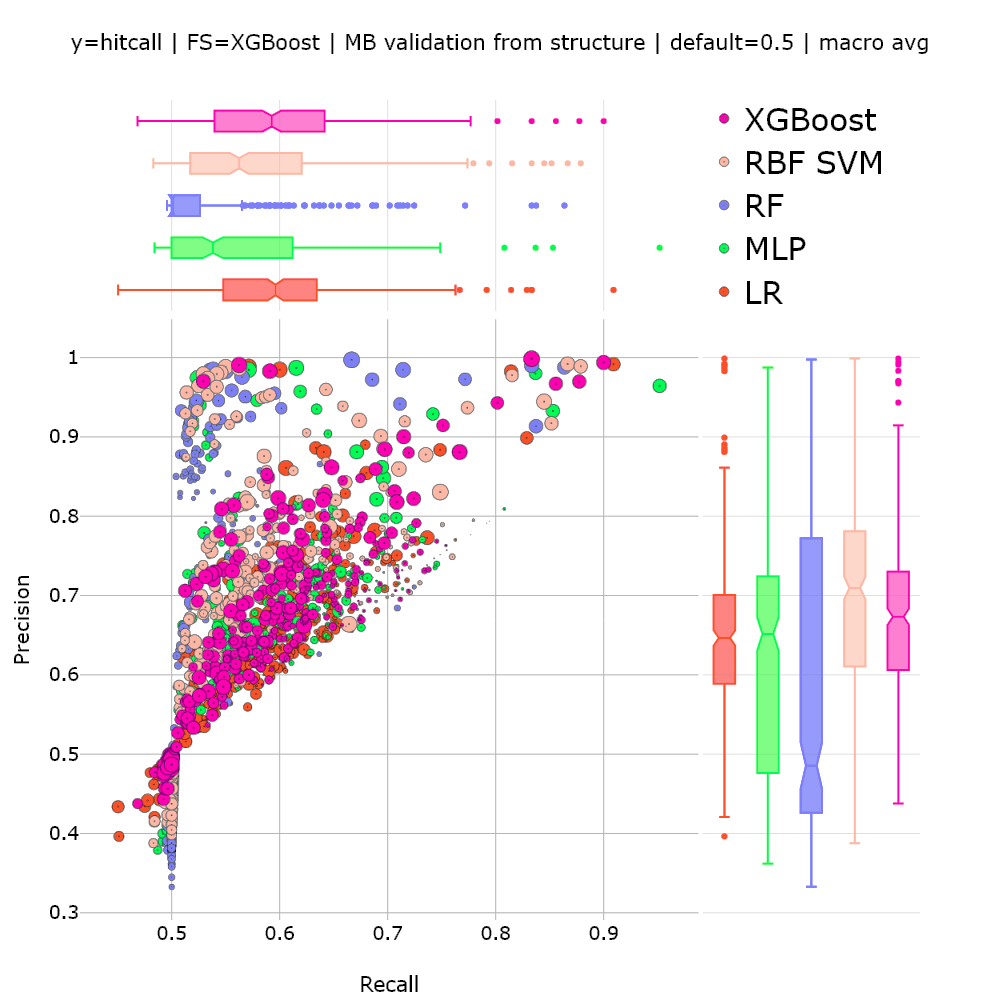
\includegraphics[width=\textwidth]{generated_results/hitcall_classification_Feature_Selection_XGBClassifier_mb_val_structure_default_macro_avg.png}
      \caption{}
  \label{fig:hitcall_classification_Feature_Selection_XGBClassifier_mb_val_structure_default_macro_avg}
  \end{subfigure}
  \hfill
  \begin{subfigure}[b]{0.495\textwidth}
      \centering
      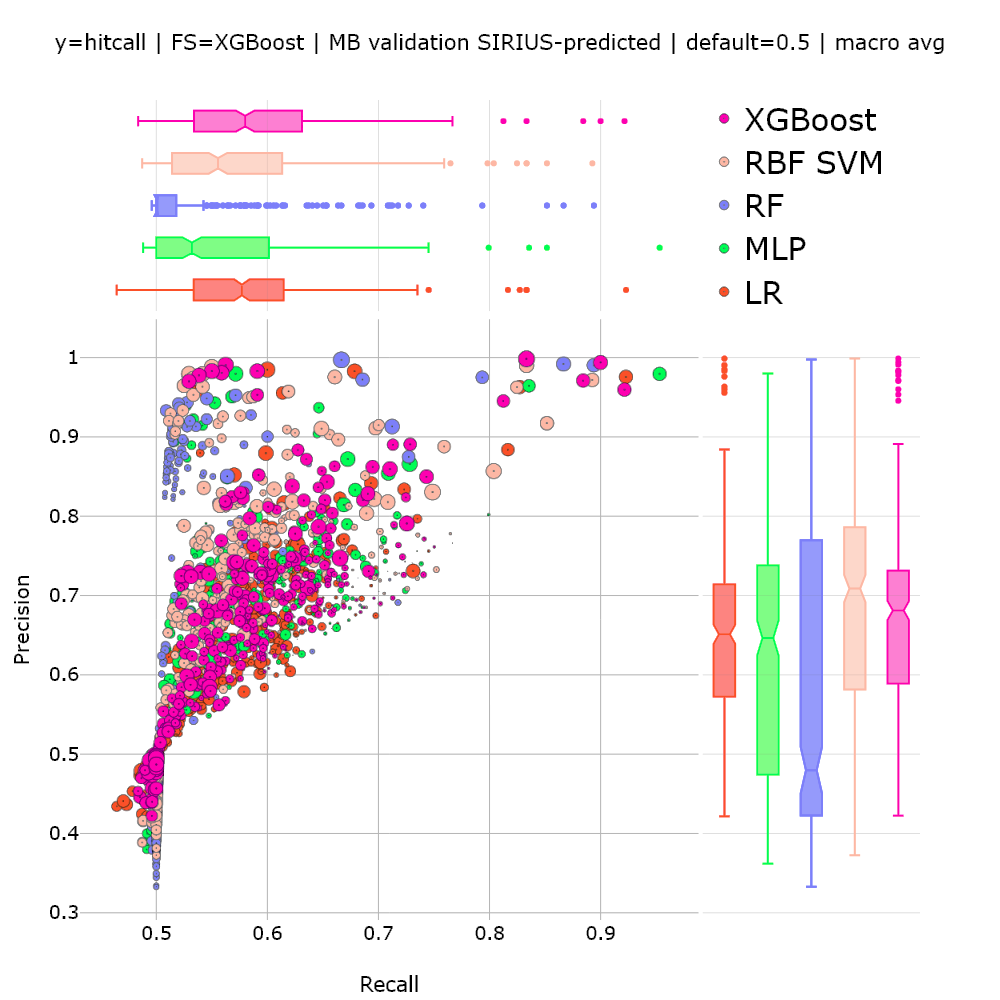
\includegraphics[width=\textwidth]{generated_results/hitcall_classification_Feature_Selection_XGBClassifier_mb_val_sirius_default_macro_avg.png}
      \caption{}
      \label{fig:hitcall_classification_Feature_Selection_XGBClassifier_mb_val_sirius_default_macro_avg}
  \end{subfigure}
  \caption{Comparison of precision and recall for five different estimators across a total of 345 evaluated assay endpoints. MassBank validation with fingerprints from chemical structure (a) and SIRIUS-predicted fingerprints (b), $default = 0.5$ threshold, macro averaged metrics. Larger marker size indicate a larger relative imbalance between the support for negative and positive compounds, normalized across all assay endpoints. The marginal boxplots illustrate the metric distribution across the target assay endpoint models (median, first quartile, third quartile, range-whiskers and outlieres).}
  \label{fig:hitcall_classification_Feature_Selection_XGBClassifier_mb_val_default_macro_avg}
\end{figure}

\begin{longtable}{llllllll}
\caption{Median Performance Metrics belonging to Figure~\ref{fig:hitcall_classification_Feature_Selection_XGBClassifier_mb_val_structure_default_macro_avg}.}\label{tab:table:hitcall_classification_feature_selection_xgbclassifier_mb_val_structure_default_macro_avg}\\
\toprule
\midrule
\small Estimator & \small Precision & \small Recall & \small F1 & \small Acc. & \small Bal. Acc. & \small ROC-AUC & \small PR-AUC\\
\hline
LR & 0.647 & 0.596 & 0.605 & 0.816 & 0.596 & 0.707 & 0.411\\
MLP & 0.651 & 0.538 & 0.530 & 0.829 & 0.538 & 0.671 & 0.363\\
RBF SVM & 0.709 & 0.562 & 0.570 & 0.835 & 0.562 & 0.738 & 0.455\\
RF & 0.486 & 0.500 & 0.474 & 0.829 & 0.500 & 0.731 & 0.436\\
XGBoost & 0.673 & 0.593 & 0.607 & 0.823 & 0.593 & 0.736 & 0.451\\
\bottomrule
\end{longtable}
\begin{longtable}{llllllll}
\caption{Median Performance Metrics belonging to~\ref{fig:hitcall_classification_Feature_Selection_XGBClassifier_mb_val_sirius_default_macro_avg}.}\label{tab:table:hitcall_classification_feature_selection_xgbclassifier_mb_val_sirius_default_macro_avg}\\
\toprule
\midrule
\small Estimator & \small Precision & \small Recall & \small F1 & \small Acc. & \small Bal. Acc. & \small ROC-AUC & \small PR-AUC\\
\hline
LR & 0.651 & 0.577 & 0.587 & 0.820 & 0.577 & 0.693 & 0.385\\
MLP & 0.646 & 0.532 & 0.519 & 0.829 & 0.532 & 0.668 & 0.355\\
RBF SVM & 0.709 & 0.556 & 0.559 & 0.834 & 0.556 & 0.726 & 0.448\\
RF & 0.480 & 0.500 & 0.471 & 0.829 & 0.500 & 0.727 & 0.433\\
XGBoost & 0.681 & 0.580 & 0.594 & 0.829 & 0.580 & 0.721 & 0.441\\
\bottomrule
\end{longtable}
\newpage

\begin{figure}[htbp]
  \centering
  \begin{subfigure}[b]{0.495\textwidth}
      \centering
      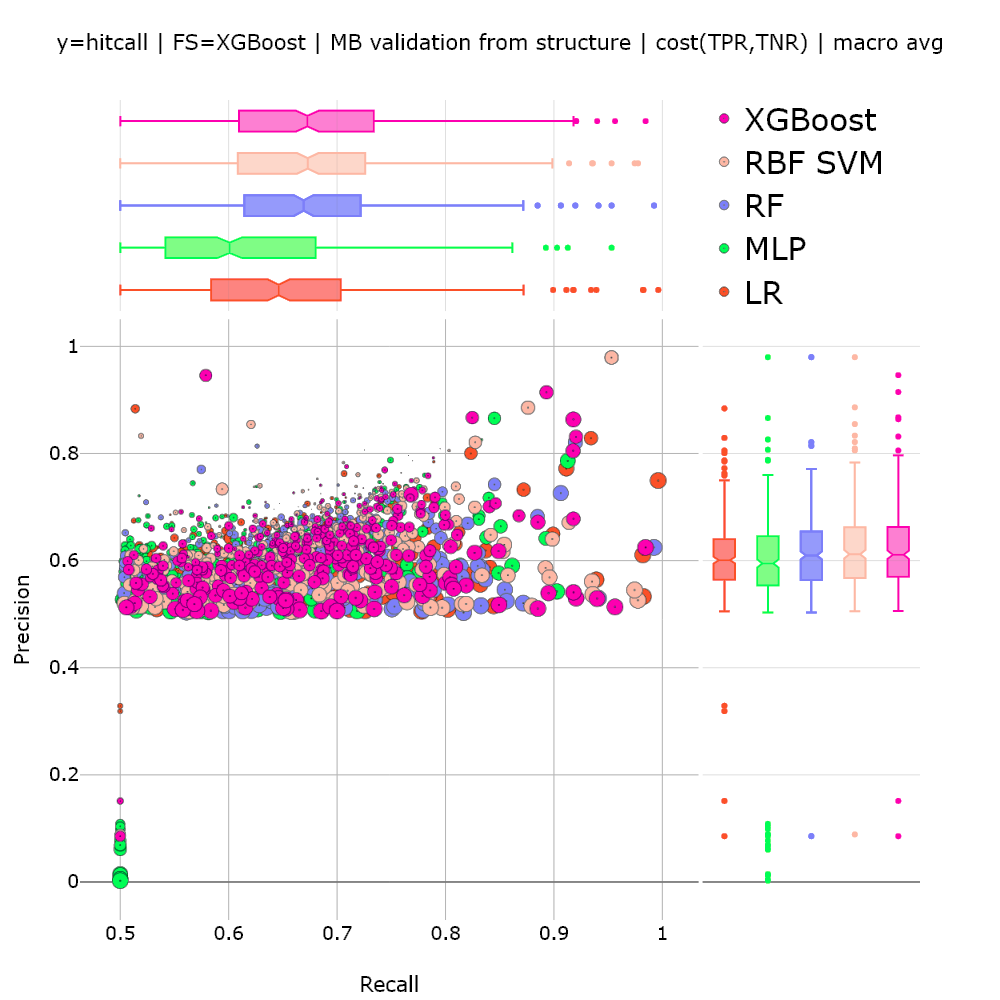
\includegraphics[width=\textwidth]{generated_results/hitcall_classification_Feature_Selection_XGBClassifier_mb_val_structure_optimal_macro_avg.png}
      \caption{}
  \label{fig:hitcall_classification_Feature_Selection_XGBClassifier_mb_val_structure_optimal_macro_avg}
  \end{subfigure}
  \hfill
  \begin{subfigure}[b]{0.495\textwidth}
      \centering
      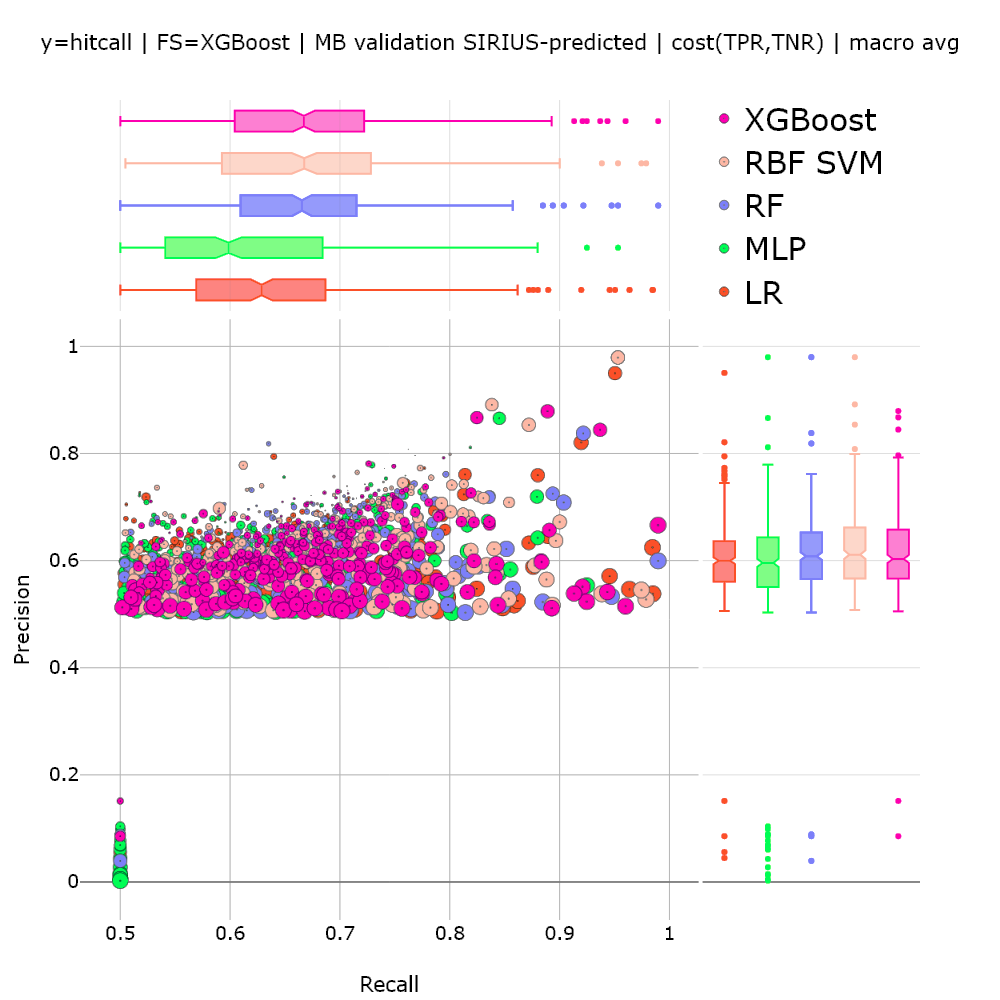
\includegraphics[width=\textwidth]{generated_results/hitcall_classification_Feature_Selection_XGBClassifier_mb_val_sirius_optimal_macro_avg.png}
      \caption{}
      \label{fig:hitcall_classification_Feature_Selection_XGBClassifier_mb_val_sirius_optimal_macro_avg}
  \end{subfigure}
  \caption{Comparison of precision and recall for five different estimators across a total of 345 evaluated assay endpoints. MassBank validation with fingerprints from chemical structure (a) and SIRIUS-predicted fingerprints (b), $\text{cost}(TPR, TNR) = 2 * (1 - TPR) + FPR$ threshold, macro averaged metrics. Larger marker size indicate a larger relative imbalance between the support for negative and positive compounds, normalized across all assay endpoints. The marginal boxplots illustrate the metric distribution across the target assay endpoint models (median, first quartile, third quartile, range-whiskers and outlieres). The tables below provide the median metrics for the estimators across all target assay endpoint models.}
  \label{fig:hitcall_classification_Feature_Selection_XGBClassifier_mb_val_optimal_macro_avg}
\end{figure}

\begin{longtable}{llllllll}
\caption{Median Performance Metrics belonging to Figure~\ref{fig:hitcall_classification_Feature_Selection_XGBClassifier_mb_val_structure_optimal_macro_avg}.}\label{tab:table:hitcall_classification_feature_selection_xgbclassifier_mb_val_structure_optimal_macro_avg}\\
\toprule
\midrule
\small Estimator & \small Precision & \small Recall & \small F1 & \small Acc. & \small Bal. Acc. & \small ROC-AUC & \small PR-AUC\\
\hline
LR & 0.601 & 0.646 & 0.470 & 0.503 & 0.596 & 0.707 & 0.411\\
MLP & 0.595 & 0.601 & 0.386 & 0.407 & 0.538 & 0.671 & 0.363\\
RBF SVM & 0.612 & 0.673 & 0.516 & 0.559 & 0.562 & 0.738 & 0.455\\
RF & 0.610 & 0.669 & 0.507 & 0.548 & 0.500 & 0.731 & 0.436\\
XGBoost & 0.611 & 0.673 & 0.511 & 0.563 & 0.593 & 0.736 & 0.451\\
\bottomrule
\end{longtable}
\begin{longtable}{llllllll}
\caption{Median Performance Metrics belonging to~\ref{fig:hitcall_classification_Feature_Selection_XGBClassifier_mb_val_sirius_optimal_macro_avg}.}\label{tab:table:hitcall_classification_feature_selection_xgbclassifier_mb_val_sirius_optimal_macro_avg}\\
\toprule
\midrule
\small Estimator & \small Precision & \small Recall & \small F1 & \small Acc. & \small Bal. Acc. & \small ROC-AUC & \small PR-AUC\\
\hline
LR & 0.600 & 0.629 & 0.432 & 0.458 & 0.577 & 0.693 & 0.385\\
MLP & 0.596 & 0.599 & 0.373 & 0.415 & 0.532 & 0.668 & 0.355\\
RBF SVM & 0.611 & 0.668 & 0.493 & 0.559 & 0.556 & 0.726 & 0.448\\
RF & 0.608 & 0.665 & 0.499 & 0.534 & 0.500 & 0.727 & 0.433\\
XGBoost & 0.603 & 0.667 & 0.502 & 0.539 & 0.580 & 0.721 & 0.441\\
\bottomrule
\end{longtable}
\newpage

\begin{figure}
  \centering
  \begin{subfigure}[b]{0.495\textwidth}
      \centering
      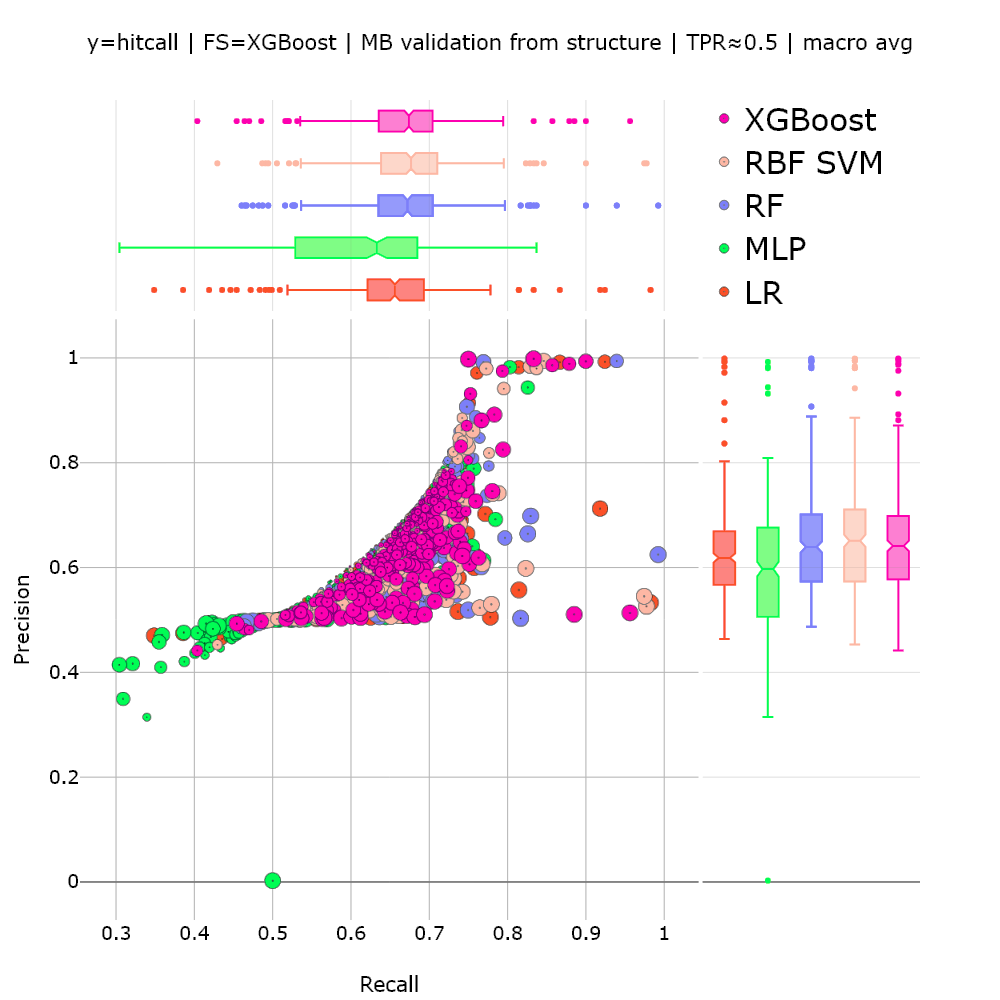
\includegraphics[width=\textwidth]{generated_results/hitcall_classification_Feature_Selection_XGBClassifier_mb_val_structure_tpr_macro_avg.png}
      \caption{}
  \label{fig:hitcall_classification_Feature_Selection_XGBClassifier_mb_val_structure_tpr_macro_avg}
  \end{subfigure}
  \hfill
  \begin{subfigure}[b]{0.495\textwidth}
      \centering
      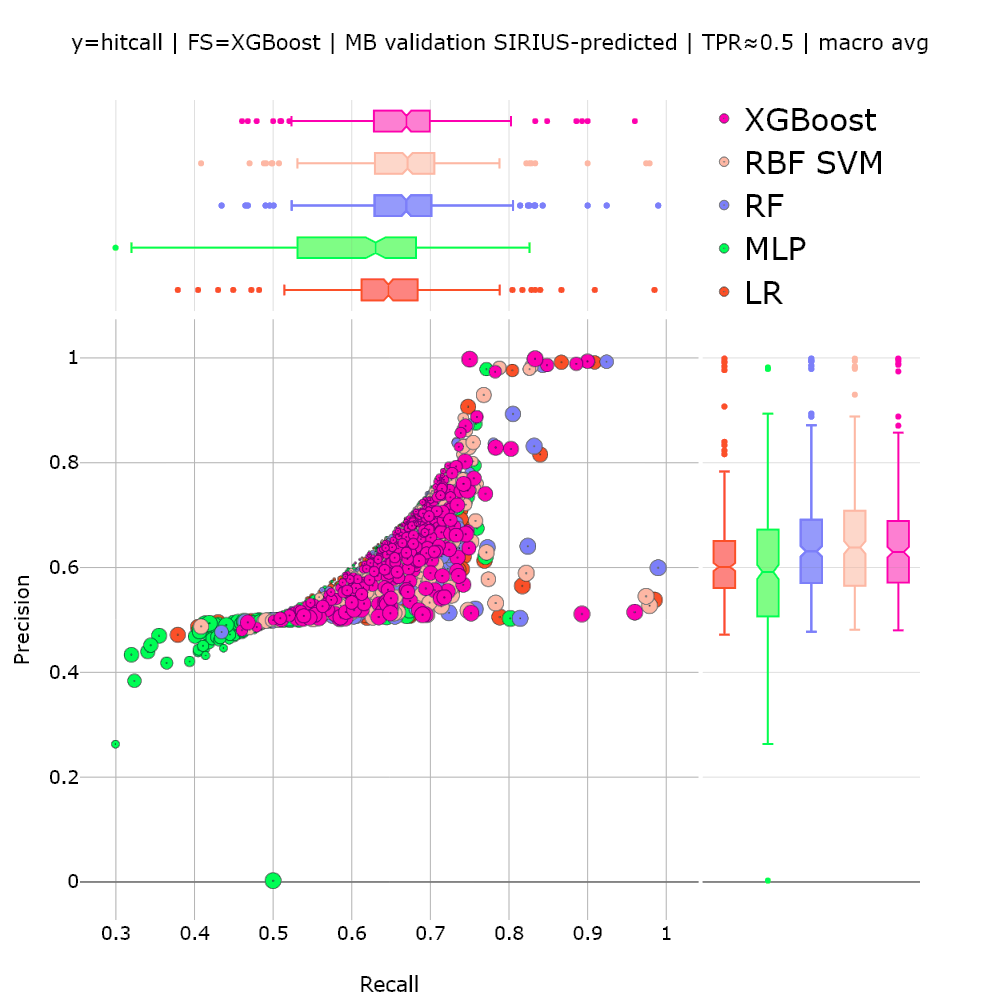
\includegraphics[width=\textwidth]{generated_results/hitcall_classification_Feature_Selection_XGBClassifier_mb_val_sirius_tpr_macro_avg.png}
      \caption{}
      \label{fig:hitcall_classification_Feature_Selection_XGBClassifier_mb_val_sirius_tpr_macro_avg}
  \end{subfigure}
  \caption{Comparison of precision and recall for five different estimators across a total of 345 evaluated assay endpoints. MassBank validation with fingerprints from chemical structure (a) and SIRIUS-predicted fingerprints (b), $TPR \simeq 0.5$ threshold, macro averaged metrics. Larger marker size indicate a larger relative imbalance between the support for negative and positive compounds, normalized across all assay endpoints. The marginal boxplots illustrate the metric distribution across the target assay endpoint models (median, first quartile, third quartile, range-whiskers and outlieres). The tables below provide the median metrics for the estimators across all target assay endpoint models.}
  \label{fig:hitcall_classification_Feature_Selection_XGBClassifier_mb_val_tpr_macro_avg}
\end{figure}

\begin{longtable}{llllllll}
\caption{Median Performance Metrics belonging to Figure~\ref{fig:hitcall_classification_Feature_Selection_XGBClassifier_mb_val_structure_tpr_macro_avg}.}\label{tab:table:hitcall_classification_feature_selection_xgbclassifier_mb_val_structure_tpr_macro_avg}\\
\toprule
\midrule
\small Estimator & \small Precision & \small Recall & \small F1 & \small Acc. & \small Bal. Acc. & \small ROC-AUC & \small PR-AUC\\
\hline
LR & 0.618 & 0.656 & 0.626 & 0.727 & 0.596 & 0.707 & 0.411\\
MLP & 0.597 & 0.633 & 0.605 & 0.683 & 0.538 & 0.671 & 0.363\\
RBF SVM & 0.651 & 0.677 & 0.656 & 0.754 & 0.562 & 0.738 & 0.455\\
RF & 0.639 & 0.672 & 0.647 & 0.750 & 0.500 & 0.731 & 0.436\\
XGBoost & 0.641 & 0.674 & 0.649 & 0.754 & 0.593 & 0.736 & 0.451\\
\bottomrule
\end{longtable}
\begin{longtable}{llllllll}
\caption{Median Performance Metrics belonging to Figure~\ref{fig:hitcall_classification_Feature_Selection_XGBClassifier_mb_val_sirius_tpr_macro_avg}.}\label{tab:table:hitcall_classification_feature_selection_xgbclassifier_mb_val_sirius_tpr_macro_avg}\\
\toprule
\midrule
\small Estimator & \small Precision & \small Recall & \small F1 & \small Acc. & \small Bal. Acc. & \small ROC-AUC & \small PR-AUC\\
\hline
LR & 0.601 & 0.647 & 0.608 & 0.711 & 0.577 & 0.693 & 0.385\\
MLP & 0.592 & 0.630 & 0.596 & 0.676 & 0.532 & 0.668 & 0.355\\
RBF SVM & 0.638 & 0.671 & 0.644 & 0.749 & 0.556 & 0.726 & 0.448\\
RF & 0.631 & 0.669 & 0.638 & 0.743 & 0.500 & 0.727 & 0.433\\
XGBoost & 0.629 & 0.670 & 0.638 & 0.743 & 0.580 & 0.721 & 0.441\\
\bottomrule
\end{longtable}
\newpage

\begin{figure}[htbp]
  \centering
  \begin{subfigure}[b]{0.495\textwidth}
      \centering
      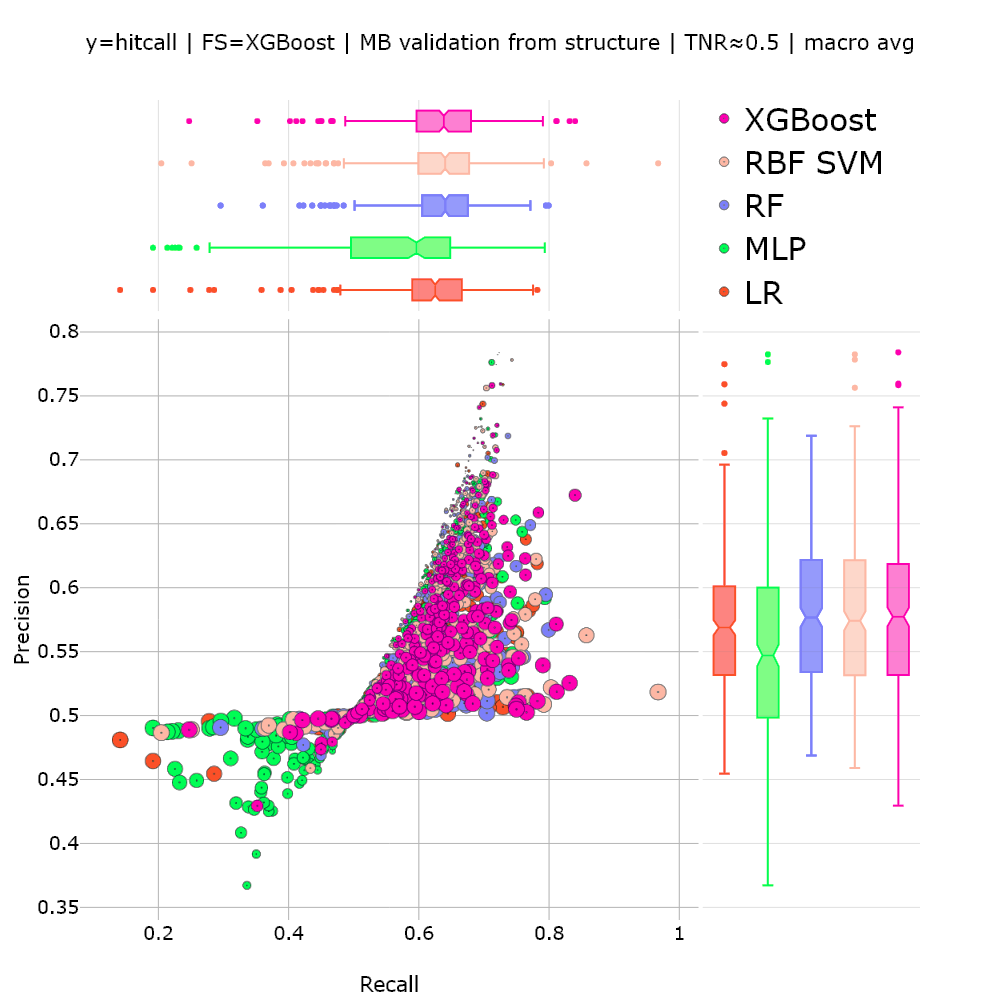
\includegraphics[width=\textwidth]{generated_results/hitcall_classification_Feature_Selection_XGBClassifier_mb_val_structure_tnr_macro_avg.png}
      \caption{}
  \label{fig:hitcall_classification_Feature_Selection_XGBClassifier_mb_val_structure_tnr_macro_avg}
  \end{subfigure}
  \hfill
  \begin{subfigure}[b]{0.495\textwidth}
      \centering
      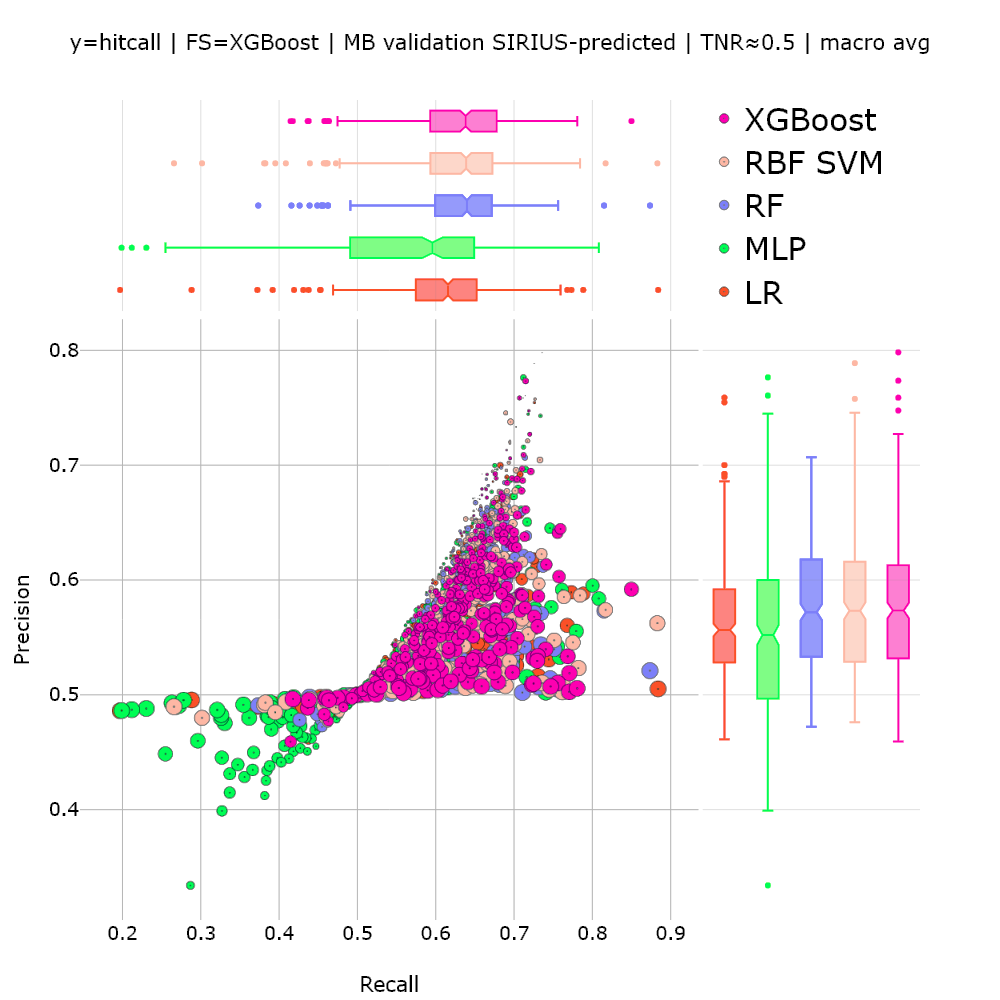
\includegraphics[width=\textwidth]{generated_results/hitcall_classification_Feature_Selection_XGBClassifier_mb_val_sirius_tnr_macro_avg.png}
      \caption{}
      \label{fig:hitcall_classification_Feature_Selection_XGBClassifier_mb_val_sirius_tnr_macro_avg}
  \end{subfigure}
  \caption{Comparison of precision and recall for five different estimators across a total of 345 evaluated assay endpoints. MassBank validation with fingerprints from chemical structure (a) and SIRIUS-predicted fingerprints (b), $TNR \simeq 0.5$ threshold, macro averaged metrics. Larger marker size indicate a larger relative imbalance between the support for negative and positive compounds, normalized across all assay endpoints. The marginal boxplots illustrate the metric distribution across the target assay endpoint models (median, first quartile, third quartile, range-whiskers and outlieres). The tables below provide the median metrics for the estimators across all target assay endpoint models.}
  \label{fig:hitcall_classification_Feature_Selection_XGBClassifier_mb_val_tnr_macro_avg}
\end{figure}

\begin{longtable}{llllllll}
\caption{Median Performance Metrics belonging to Figure~\ref{fig:hitcall_classification_Feature_Selection_XGBClassifier_mb_val_structure_tnr_macro_avg}.}\label{tab:table:hitcall_classification_feature_selection_xgbclassifier_mb_val_structure_tnr_macro_avg}\\
\toprule
\midrule
\small Estimator & \small Precision & \small Recall & \small F1 & \small Acc. & \small Bal. Acc. & \small ROC-AUC & \small PR-AUC\\
\hline
LR & 0.569 & 0.625 & 0.509 & 0.552 & 0.596 & 0.707 & 0.411\\
MLP & 0.547 & 0.596 & 0.478 & 0.537 & 0.538 & 0.671 & 0.363\\
RBF SVM & 0.574 & 0.640 & 0.509 & 0.556 & 0.562 & 0.738 & 0.455\\
RF & 0.577 & 0.641 & 0.514 & 0.555 & 0.500 & 0.731 & 0.436\\
XGBoost & 0.577 & 0.638 & 0.509 & 0.553 & 0.593 & 0.736 & 0.451\\
\bottomrule
\end{longtable}
\begin{longtable}{llllllll}
\caption{Median Performance Metrics belonging to~\ref{fig:hitcall_classification_Feature_Selection_XGBClassifier_mb_val_sirius_tnr_macro_avg}.}\label{tab:table:hitcall_classification_feature_selection_xgbclassifier_mb_val_sirius_tnr_macro_avg}\\
\toprule
\midrule
\small Estimator & \small Precision & \small Recall & \small F1 & \small Acc. & \small Bal. Acc. & \small ROC-AUC & \small PR-AUC\\
\hline
LR & 0.557 & 0.616 & 0.497 & 0.543 & 0.577 & 0.693 & 0.385\\
MLP & 0.552 & 0.596 & 0.481 & 0.541 & 0.532 & 0.668 & 0.355\\
RBF SVM & 0.573 & 0.639 & 0.506 & 0.555 & 0.556 & 0.726 & 0.448\\
RF & 0.572 & 0.640 & 0.507 & 0.553 & 0.500 & 0.727 & 0.433\\
XGBoost & 0.573 & 0.638 & 0.507 & 0.553 & 0.580 & 0.721 & 0.441\\
\bottomrule
\end{longtable}

\newpage
\subsection{Feature Importance}\label{sec:feature_importance}
Evaluating the importance of fingerprint features allows for the exploration of the relation between molecular substructures within compounds and their potential for toxicity. High feature importance indicates a significant association between the presence or absence of the substructure and its impact on predicting toxicity.
We have gathered feature importance scores for all assay endpoints from their respective trained XGBoost and random forest classifiers associated with their feature selection models. As an illustration, we can visualize the top $N$ features for each assay endpoint, as demonstrated in Figure~\ref{fig:feature_importance} for the case where $N=10$ an the XGBoost classifier.

To compare important fingerprint features between both independent classifiers, we analyzed common features among their top 10 lists. Features appearing in fewer than 10 endpoints were removed, reducing the set to 119 features. The resulting presence matrix represents the constrained feature space with $345 * 119 = 41'055$ entries. The combined total of these features present in both the obtained presence matrices for XGBoost ($1'520$, Figure~\ref{fig:Feature_Selection_XGBClassifier__Feature_Selection_XGBClassifier_feature_importance}) and the random forest ($2'626$, Figure~\ref{fig:Feature_Selection_RandomForestClassifier__Feature_Selection_RandomForestClassifier_feature_importance}) model amounts to $4'146$, with $722$ of these features being common to both models, as depicted in Figure~\ref{fig:matching_features}.

\begin{figure}[h]
  \centering
  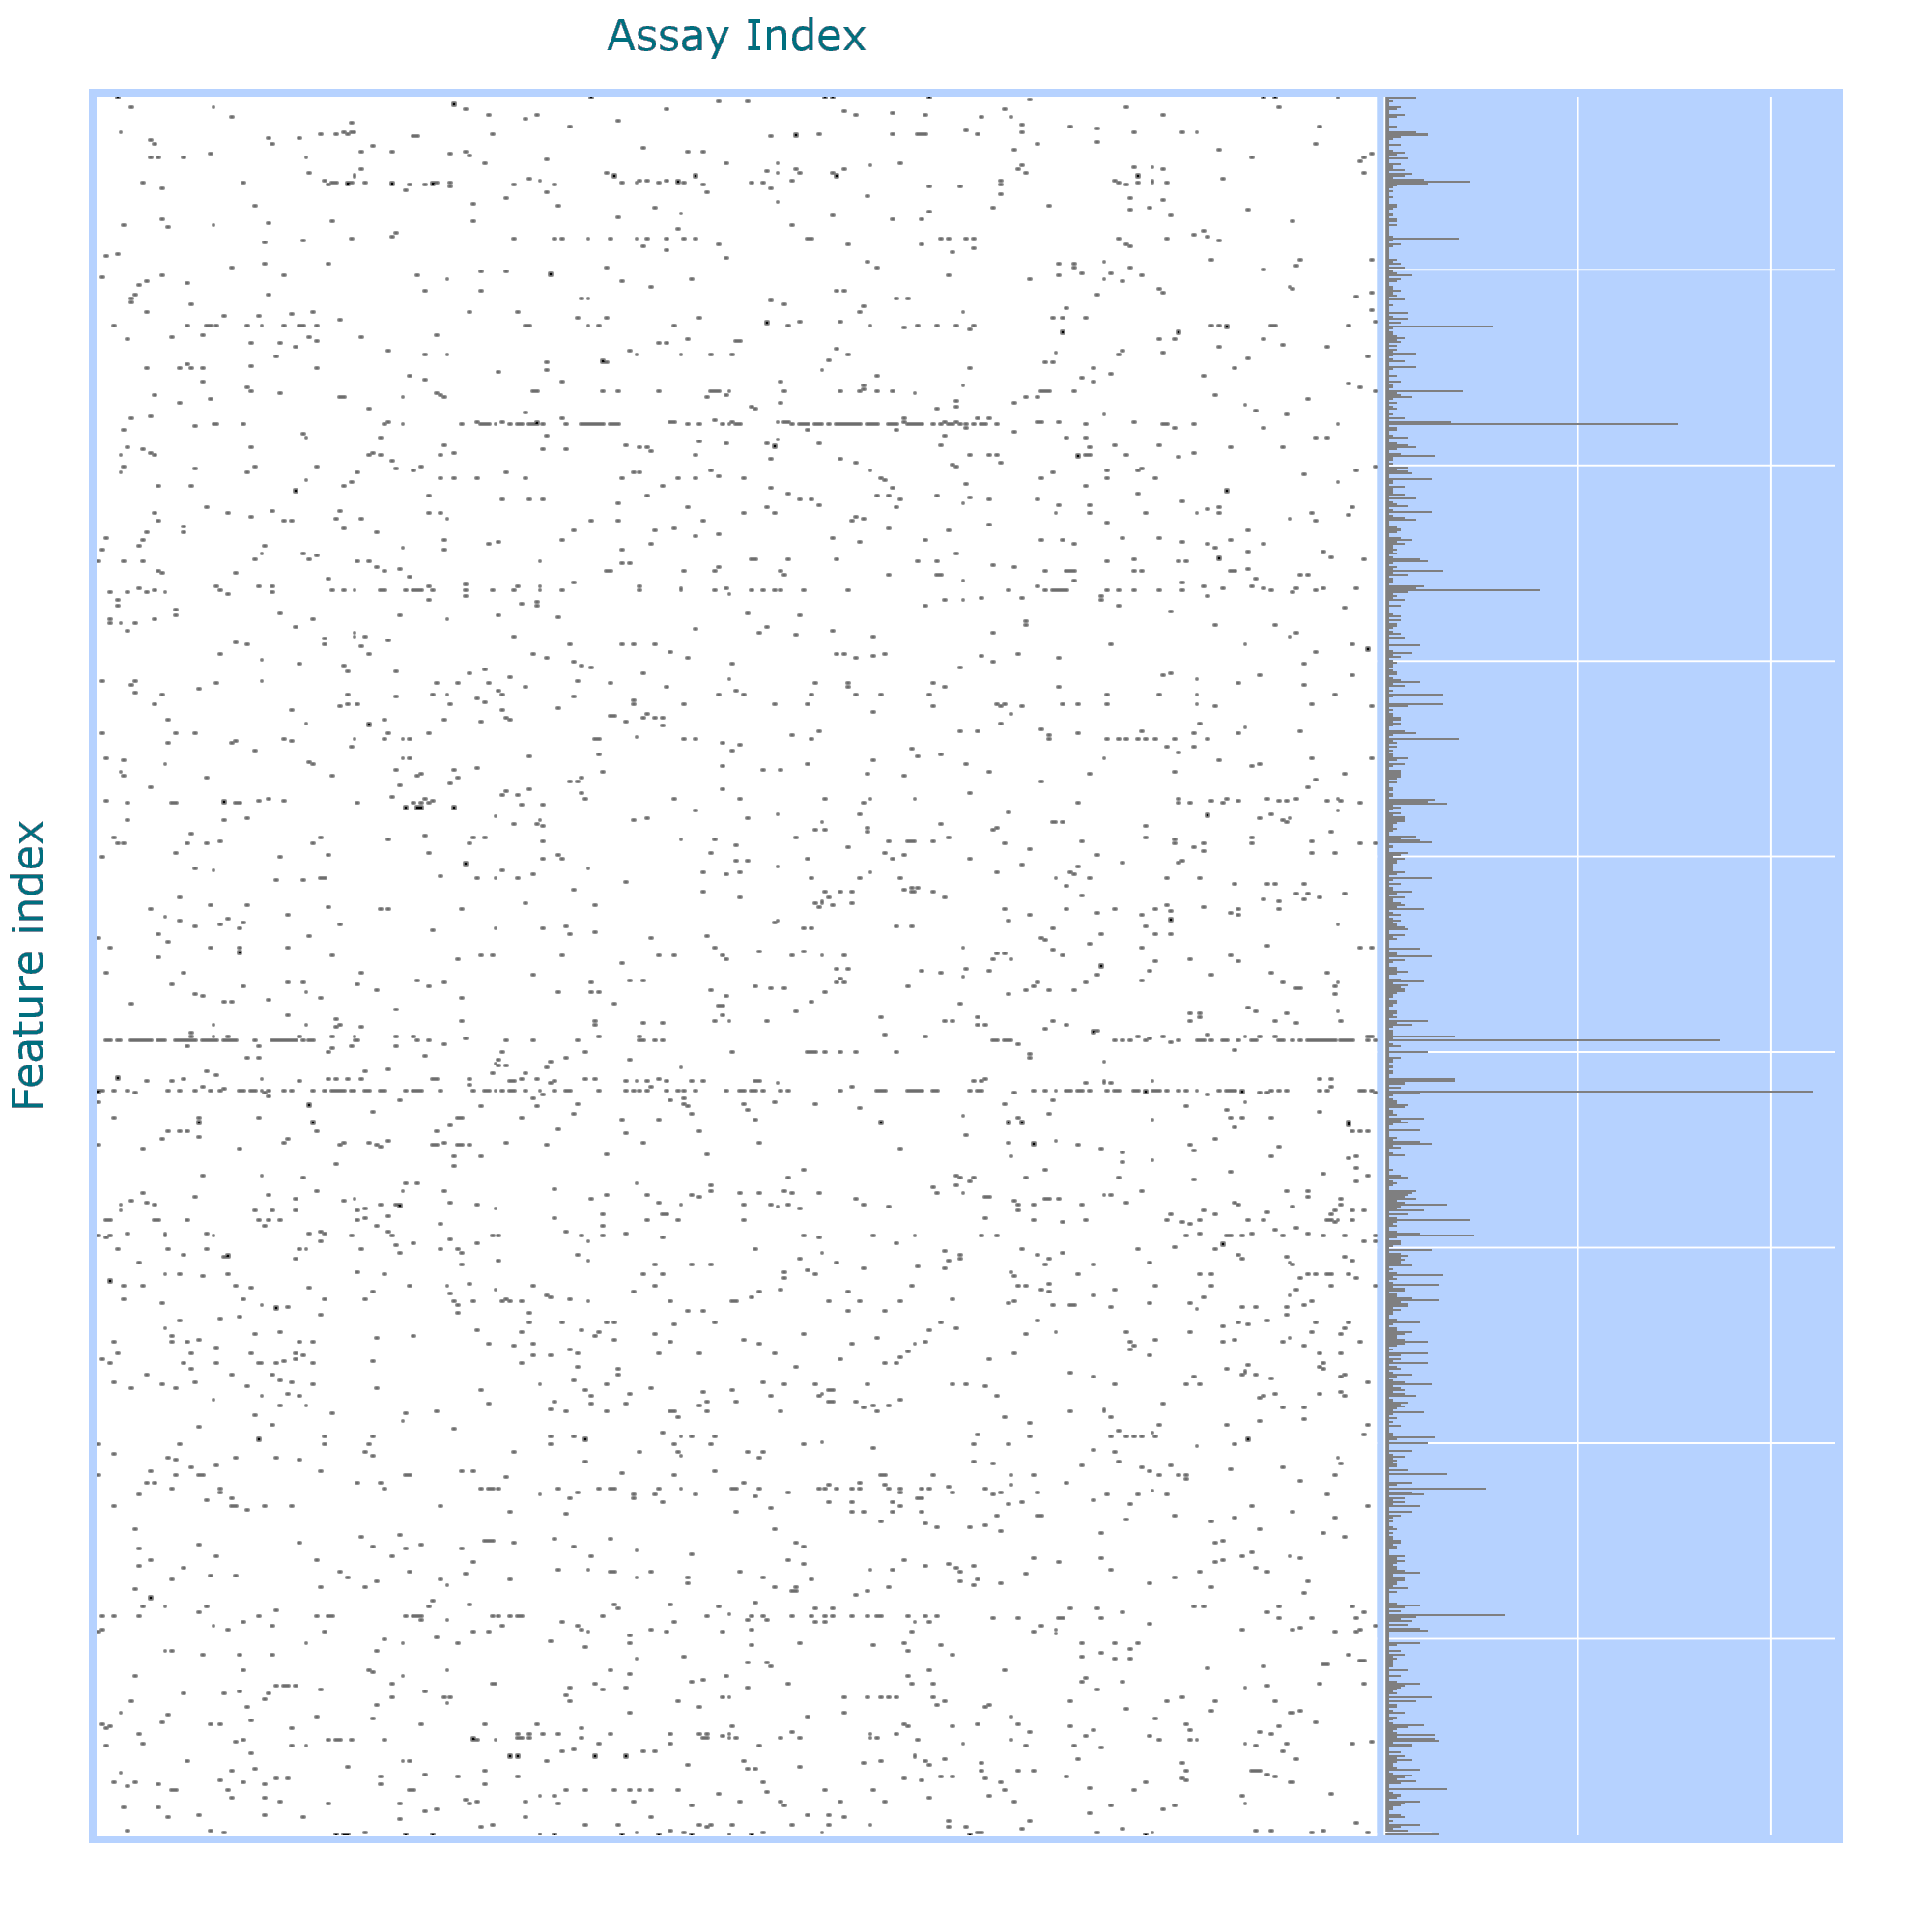
\includegraphics[width=0.68\textwidth]{figures/feature_importance.png}  
  \caption{Top 10 features across all target assay enpoints. The constrained feature space (889 features) is a product of the top 10 features specific to each assay endpoint, chosen through their respective XGBoost feature selection models. We converted the initial feature indices into a new linear index to facilitate visualization.}
~\label{fig:feature_importance} 
\end{figure}


\begin{figure}[h]
  \centering
  
\includegraphics[width=1.0\textwidth]{figures/Feature_Selection_XGBClassifier__Feature_Selection_XGBClassifier_feature_importance.png}  
  \caption{The most important features for the XGBosst classifier visualized in a presence matrix.}
~\label{fig:Feature_Selection_XGBClassifier__Feature_Selection_XGBClassifier_feature_importance} 
\end{figure}

\begin{figure}[h]
  \centering
  
\includegraphics[width=1.0\textwidth]{figures/Feature_Selection_RandomForestClassifier__Feature_Selection_RandomForestClassifier_feature_importance.png}  
  \caption{The most important features for the random forest classifier visualized in a presence matrix.}
~\label{fig:Feature_Selection_RandomForestClassifier__Feature_Selection_RandomForestClassifier_feature_importance} 
\end{figure}

\begin{figure}[h]
  \centering
  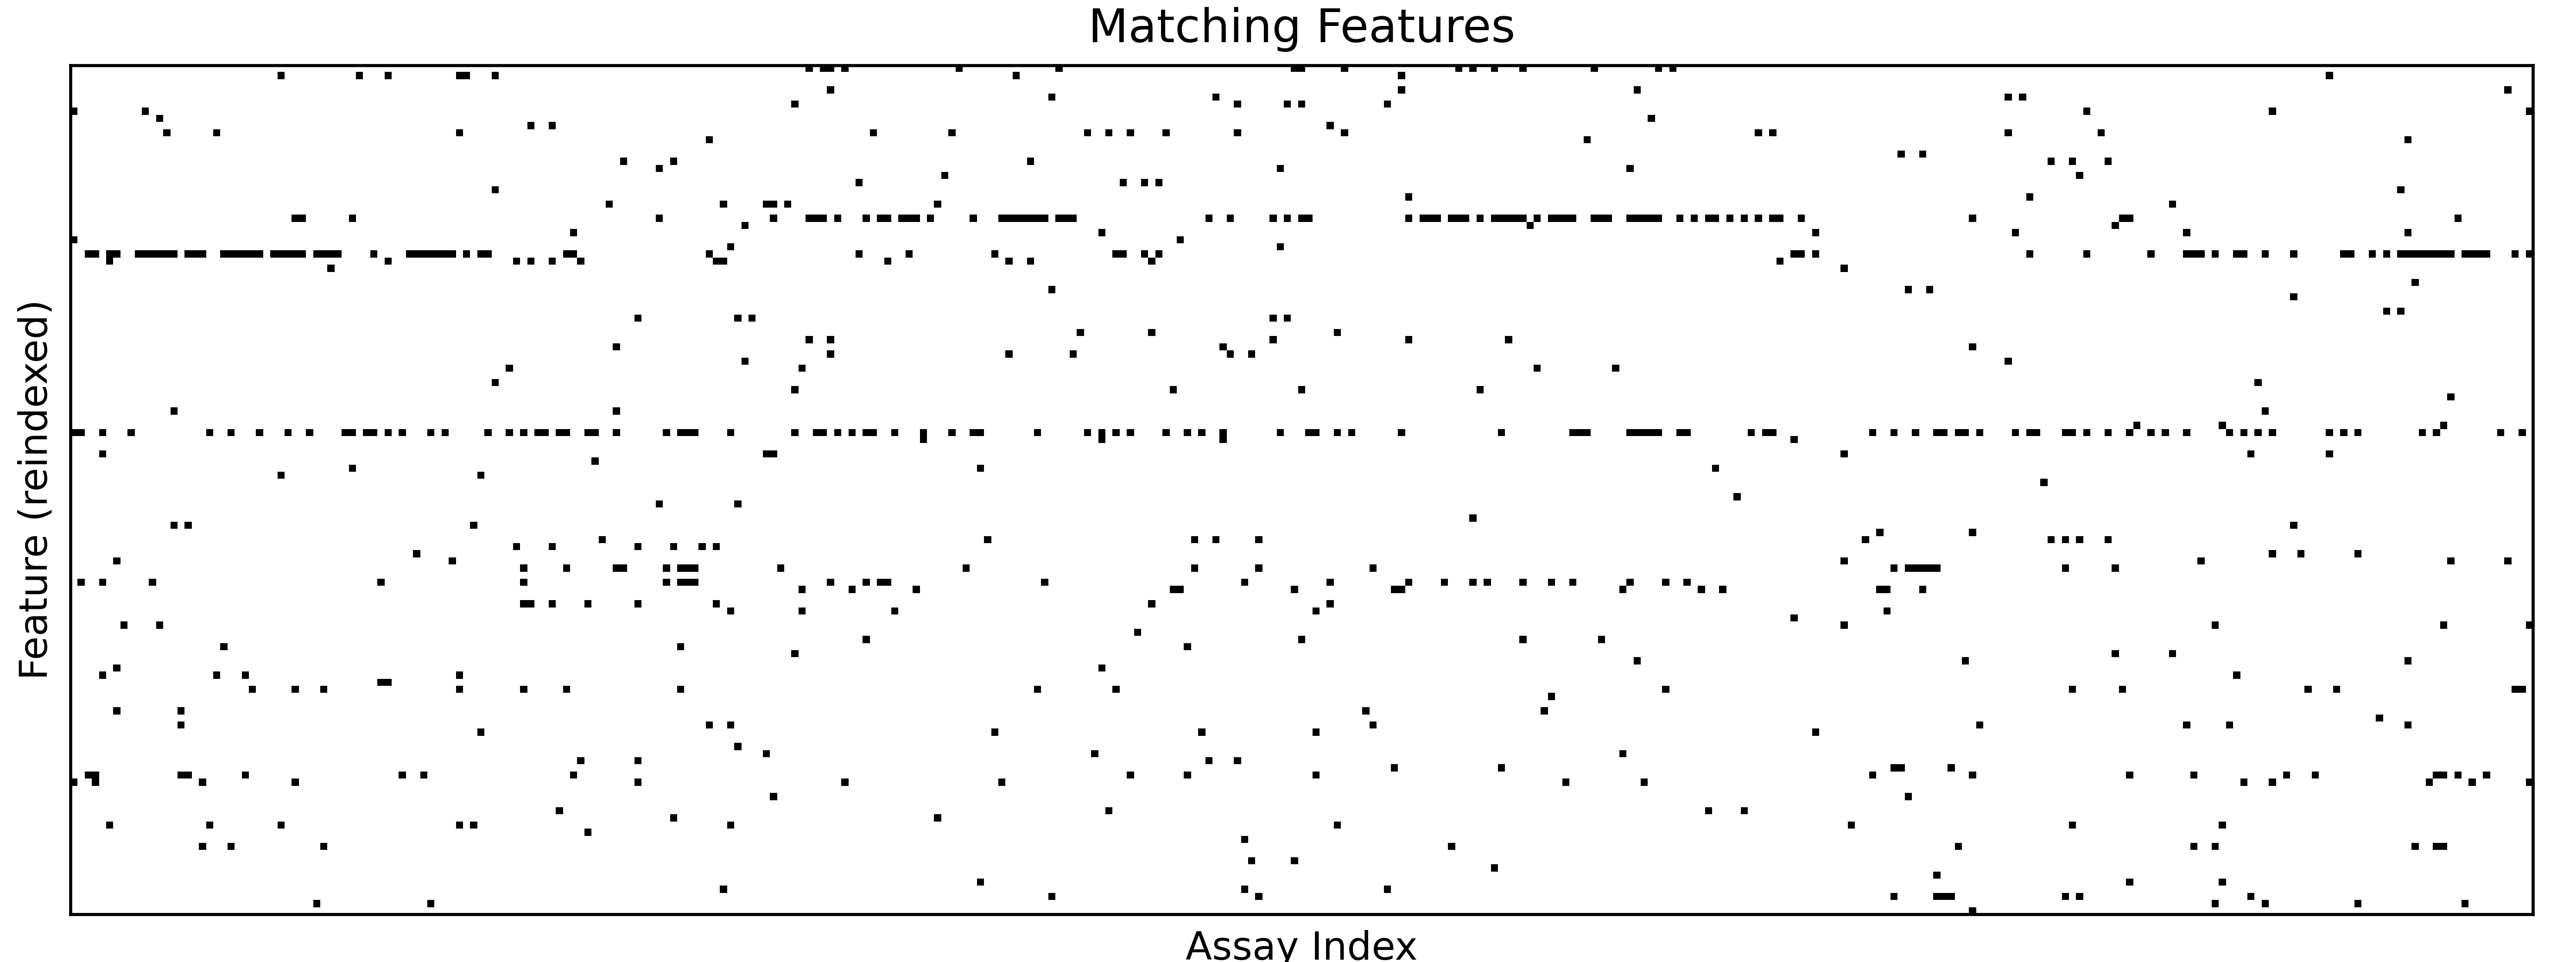
\includegraphics[width=0.97\textwidth]{figures/matching_features.png}  
  \caption{The 722 shared features within the top 10 most important features identified by both the XGBoost and random forest classifiers across the 345 target assay endpoints.}
~\label{fig:matching_features} 
\end{figure}







